\documentclass[journal]{IEEEtran}
\usepackage{amsmath,amssymb,amsfonts}
\usepackage{algorithmic}
\usepackage{algorithm}
\usepackage{array}
\usepackage[caption=false,font=footnotesize]{subfig}
\usepackage{textcomp}
\usepackage{stfloats}
\usepackage{url}
\usepackage{verbatim}
\usepackage{graphicx}
\usepackage{cite}
\usepackage{booktabs}
\usepackage{multirow}
\usepackage{tikz}
\usepackage{pgfplots}
\pgfplotsset{compat=1.18}
\usetikzlibrary{shapes.geometric, arrows, positioning, fit, calc}

\hyphenation{op-tical net-works semi-conduc-tor IEEE-Xplore}

\begin{document}

\title{Deadline-Driven Hybrid Particle Swarm Optimization for Multi-Objective Scientific Workflow Scheduling in IaaS Clouds}

\author{Sparsh~Rastogi,~\IEEEmembership{Student Member,~IEEE,}
        Nisha~Mittal,~\IEEEmembership{Student Member,~IEEE,}
        and~Prasenjit~Chanak,~\IEEEmembership{Senior Member,~IEEE}%
\thanks{Manuscript received November 10, 2026; revised January 15, 2027; accepted February 20, 2027. Date of publication March 5, 2027; date of current version March 25, 2027. This work was supported by the Department of Computer Science and Engineering, Indian Institute of Technology (BHU) Varanasi, India. \textit{(Corresponding author: Prasenjit Chanak.)}}%
\thanks{Sparsh Rastogi, Nisha Mittal, and Prasenjit Chanak are with the Department of Computer Science and Engineering, Indian Institute of Technology (BHU) Varanasi, Varanasi 221005, India (e-mail: sparsh.rastogi.cse21@itbhu.ac.in; nisha.mittal.cse21@itbhu.ac.in; prasenjit.cse@iitbhu.ac.in).}%
\thanks{Digital Object Identifier 10.1109/TCC.2027.3592044}}

\markboth{IEEE TRANSACTIONS ON CLOUD COMPUTING,~Vol.~15, No.~2,~April~2027}%
{Rastogi \MakeLowercase{\textit{et al.}}: Deadline-Driven Hybrid Particle Swarm Optimization for Scientific Workflow Scheduling}

\maketitle

\begin{abstract}
In today's era, scientific workflows play a crucial role in processing massive data volumes across scientific domains such as earthquake hazard modeling, astronomy, epigenomics, and gravitational-wave physics. Infrastructure-as-a-Service (IaaS) clouds offer on-demand elastic computing resources to execute these computational workflows. However, scheduling complex Directed Acyclic Graph (DAG) applications across heterogeneous Virtual Machines (VMs) under user-defined deadline constraints is challenging due to commercial discrete hourly billing, VM boot latencies, and tenant-side energy dissipation. Existing heuristic list schedulers are greedy and myopic, failing to account for quantum billing boundaries. Unseeded metaheuristics suffer from severe initial search dispersion, leading to high deadline violation rates under strict deadlines. Conversely, classical task duplication techniques eliminate communication bottlenecks at the expense of severe monetary cost inflation and energy waste. Therefore, this paper proposes a Deadline-Driven Hybrid Particle Swarm Optimization (DD-HPSO) algorithm for multi-objective scientific workflow scheduling in IaaS clouds. First, a Heterogeneous Earliest Finish Time (HEFT)-seeded swarm initialization mechanism with fixed topological order encoding is proposed to guarantee initial deadline feasibility and accelerate convergence. Second, a proportional sub-deadline distribution scheme is introduced to localize scheduling milestones across workflow stages. Third, a dual-constrained zero-cost critical parent duplication mechanism ($\theta_C = 0, \theta_E \le 5\%$) is proposed to opportunistically exploit idle VM slack time without inducing extra billing hours or exceeding strict energy budgets. Furthermore, Deb's feasibility rules are integrated with a normalized multi-objective fitness function to simultaneously balance financial cost, energy consumption, and makespan. Extensive simulations across 1,323 benchmark runs on standard Pegasus workflows (CyberShake, Montage, Epigenomics, and Inspiral) demonstrate that DD-HPSO achieves 100.0\% deadline feasibility, an 8.9\% average reduction in monetary cost, a 6.8\% reduction in energy consumption, and maintains makespan within 2.3\% of HEFT, while significantly outperforming state-of-the-art metaheuristics whose deadline failure rates reach up to 38.6\%.
\end{abstract}

\begin{IEEEkeywords}
Cloud computing, scientific workflow scheduling, particle swarm optimization (PSO), task duplication, deadline constraint, hourly billing, energy efficiency.
\end{IEEEkeywords}

\section{Introduction}
\IEEEPARstart{I}{nfrastructure}-as-a-Service (IaaS) cloud computing platforms have emerged as the premier computational paradigm for executing data- and compute-intensive scientific workflows \cite{topcuoglu2002heft, pegasus2015}. Modern scientific domains---including seismic hazard analysis (CyberShake), astronomical sky image mosaicking (Montage), genome sequencing (Epigenomics), and gravitational-wave detection (Inspiral/LIGO)---model complex workflows as Directed Acyclic Graphs (DAGs) \cite{pegasus2015, genez2018heft}. In these scientific workflows, nodes represent interdependent computational tasks and directed edges quantify intermediate data transfers. The primary challenge in IaaS cloud environments is mapping heterogeneous workflow tasks onto leased Virtual Machine (VM) instances to satisfy user-specified end-to-end deadlines ($D$) while simultaneously minimizing monetary leasing costs and tenant energy dissipation \cite{rodriguez2014cost, ceas2018li}.

Commercial cloud providers (e.g., Amazon EC2, Google Cloud Platform, Microsoft Azure) impose realistic operational constraints that complicate workflow scheduling. First, instances are billed in discrete time quanta $\tau$ (typically 1 hour or 3600 seconds) where any fractional usage incurs full quantum charges \cite{rodriguez2014cost}. Second, VM provisioning is not instantaneous; each instance experiences an operating system initialization and hypervisor boot latency $\beta$ (empirically measured around 97 seconds) that is billed to the tenant and consumes electrical energy \cite{rodriguez2014cost, ceas2018li}. Third, communication bandwidth across distinct VMs is finite ($B = 100$ MB/s), creating severe data transfer bottlenecks for communication-heavy workflows \cite{genez2018heft}.

To address these challenges, existing workflow scheduling literature is broadly categorized into heuristic list schedulers and stochastic metaheuristics. Priority-based list schedulers, such as the classic Heterogeneous Earliest Finish Time (HEFT) algorithm \cite{topcuoglu2002heft}, greedily minimize earliest completion times. However, HEFT ignores billing cycle boundaries and energy consumption, leading to premature provisioning of underutilized, costly VM instances. Duplication-based list schedulers, such as HEFT with Task Duplication (HEFT-TD) proposed by Genez \textit{et al.} \cite{genez2018heft}, replicate critical parent tasks on target VMs to eliminate edge transfer delays. Nevertheless, unconstrained duplication myopically prolongs VM lease durations across billing boundaries, causing catastrophic monetary cost inflation and energy wastage.

Conversely, metaheuristic algorithms, such as Particle Swarm Optimization (PSO), Genetic Algorithms (GA), and Grey Wolf Optimization (GWO), have been explored for global multi-objective exploration \cite{rodriguez2014cost, wpso2025wang, awad2026ipso}. Rodriguez and Buyya \cite{rodriguez2014cost} formulated a cost-minimizing PSO under hourly billing. Li \textit{et al.} \cite{ceas2018li} proposed Cost- and Energy-Aware Scheduling (CEAS) using sub-makespan VM downscaling. Recent 2025/2026 baselines, such as Wang \textit{et al.}'s WPSO \cite{wpso2025wang} and Awad \textit{et al.}'s IPSO-GWO \cite{awad2026ipso}, introduce interval reuse and hybridization. Despite their advancements, existing metaheuristics initialize particles uniformly at random. Under tight deadline constraints ($D = 1.2 \times M_{\text{HEFT}}$), random search particles drift into highly infeasible regions, leading to severe deadline violation rates (exceeding 25\% to 38\%). Furthermore, existing metaheuristics omit task duplication due to combinatorial complexity, leaving substantial communication delay unmitigated.

To bridge these critical gaps, this paper proposes a \textbf{Deadline-Driven Hybrid Particle Swarm Optimization (DD-HPSO)} scheduling framework for IaaS clouds. DD-HPSO combines the deterministic guarantees of HEFT with the global search power of PSO and the latency-reduction advantages of task duplication, governed by strict financial and energy constraints. The major contributions of this paper are summarized as follows:
\begin{itemize}
    \item We propose a \textbf{Hybrid Swarm Seeding and Topological Order Encoding Scheme}. By embedding the deterministic HEFT solution directly into Particle 1 and applying controlled mutation ($p_{\text{mut}} = 0.1$) to the remainder of the swarm, DD-HPSO guarantees 100.0\% initial feasibility under tight deadlines while restricting search dimensions to task-to-VM assignments.
    \item We design a \textbf{Proportional Sub-Deadline Assignment Scheme ($SD_i$)} that projects global deadline slack proportionally onto individual tasks based on their HEFT finish times, serving as an efficient local filter for duplication candidate selection.
    \item We introduce a \textbf{Sub-Deadline Triggered, Zero-Cost Critical Parent Duplication Mechanism}. Duplication is evaluated only when a task exceeds its sub-deadline ($AFT_{old} > SD_i$). Duplicates are committed if and only if they fit into existing idle slots within already-billed hourly quanta ($\theta_C = 0$) and comply with a cumulative tenant energy threshold ($\theta_E \le 5\%$).
    \item We formulate a \textbf{Normalized Multi-Objective Fitness Evaluation Function} combined with \textbf{Deb's Feasibility Comparison Rules}, simultaneously balancing monetary cost, tenant energy dissipation, and schedule makespan without requiring arbitrary penalty multipliers.
    \item We conduct extensive simulations across 1,323 runs on 21 benchmark cases derived from realistic Pegasus scientific workflows (CyberShake, Montage, Epigenomics, Inspiral). Non-parametric Wilcoxon signed-rank tests confirm statistically significant improvements over seven state-of-the-art baselines.
\end{itemize}

The remainder of this paper is organized as follows: Section II reviews related literature and contrasts existing state-of-the-art approaches. Section III details the system model, billing formulation, and energy framework. Section IV describes the proposed DD-HPSO algorithm and theoretical complexity. Section V presents empirical simulation results and statistical analysis. Finally, Section VI concludes the paper and outlines future directions.

\section{Related Work}
Scientific workflow scheduling in distributed and cloud systems has received substantial research attention. This section reviews existing approaches categorized into list-based heuristics and metaheuristic optimization frameworks.

\subsection{Priority- and List-Based Workflow Schedulers}
List scheduling heuristics represent the most prevalent class of deterministic workflow schedulers due to their low computational complexity $\mathcal{O}(|V_{\text{tasks}}|^2 \cdot K)$. The foundational HEFT algorithm by Topcuoglu \textit{et al.} \cite{topcuoglu2002heft} computes an upward rank ($\text{rank}_u$) for each task based on mean execution and transfer times, assigning tasks greedily to VMs that minimize Earliest Finish Time (EFT). While highly effective at makespan minimization, HEFT is oblivious to cloud-specific economic models, such as hourly billing periods and tenant-side energy costs.

To mitigate inter-VM communication overhead, task duplication heuristics have been explored. Genez \textit{et al.} \cite{genez2018heft} proposed HEFT with Task Duplication (HEFT-TD) and Lookahead-TD, wherein critical parent tasks are duplicated into available idle gaps of target VMs to eliminate network transfer latency. However, HEFT-TD optimizes solely for makespan without monetary cost constraints. In commercial clouds, duplicating compute tasks frequently extends the VM leasing interval past an hourly boundary ($T_{\text{leased}} > \tau$), triggering full additional hourly charges. Recently, Cheng \textit{et al.} (2025) \cite{cheng2025pacm} introduced the Path-Aware Cost Minimization (PACM) heuristic, which identifies non-critical paths to scale down VM speeds. Although PACM achieves good cost reduction, its deterministic greedy decisions cannot escape local optima in complex DAG topologies.

\subsection{Metaheuristic and Hybrid Workflow Schedulers}
To achieve multi-objective trade-offs, stochastic metaheuristics have been widely adopted. Rodriguez and Buyya \cite{rodriguez2014cost} formulated a cost-minimizing PSO scheduler for IaaS clouds incorporating hourly billing periods and VM boot delays. Their model employed Deb's feasibility rules to handle deadlines. However, because their swarm was initialized purely at random, convergence on large workflows was slow, and particles frequently failed to discover feasible schedules when deadlines were set tight.

Li \textit{et al.} \cite{ceas2018li} developed the Cost- and Energy-Aware Scheduling (CEAS) algorithm, which computes sub-makespans across workflow levels and greedily maps tasks to the slowest feasible VM instance. Nevertheless, in non-DVFS multi-tenant environments, aggressive downscaling causes severe cascading delays that violate tight deadlines.

More recently, hybrid and advanced metaheuristics have been proposed. Wang \textit{et al.} (2025) \cite{wpso2025wang} proposed an improved PSO incorporating Latest Finish Time (LFT) filtering and billing interval reuse (WPSO) to minimize workflow rental costs. Awad \textit{et al.} (2026) \cite{awad2026ipso} presented a hybrid IPSO-GWO metaheuristic combining the exploration capability of Grey Wolf Optimizer (GWO) with PSO exploitation to balance cost and makespan. Despite these innovations, existing metaheuristic approaches share two persistent vulnerabilities: (i) random swarm initialization causes significant deadline failures under tight deadlines ($D = 1.2 \times M_{\text{HEFT}}$), and (ii) they omit task duplication, leaving significant communication latency on inter-VM data edges. Table~\ref{tab:sota_comparison} presents an exhaustive comparison of the state-of-the-art workflow scheduling approaches against the proposed DD-HPSO framework.

\begin{table*}[t]
\centering
\caption{Evaluation of State-of-the-Art Workflow Scheduling Approaches}
\label{tab:sota_comparison}
\resizebox{\textwidth}{!}{%
\begin{tabular}{lllccccccc}
\toprule
\textbf{Author \& Year} & \textbf{Algorithm / Technique} & \textbf{Primary Contribution} & \textbf{Heterogeneity} & \textbf{Deadline-Aware} & \textbf{Duplication} & \textbf{Hourly Billing} & \textbf{Energy-Aware} & \textbf{Initial Seeding} & \textbf{Tight Feasibility} \\
\midrule
Topcuoglu \textit{et al.} [1], 2002 & HEFT & Upward rank list scheduling & Yes & No & No & No & No & Deterministic & 100.0\% (Reference) \\
Genez \textit{et al.} [2], 2018 & HEFT-TD & Critical-parent task duplication & Yes & No & Yes & No & No & Deterministic & 100.0\% \\
Rodriguez \& Buyya [3], 2014 & Rodriguez PSO & Cost minimization under hourly billing & Yes & Yes & No & Yes & No & Random & 61.4\% \\
Li \textit{et al.} [4], 2018 & CEAS (without DVFS) & Sub-makespan VM downscaling & Yes & Yes & No & Yes & Yes & Deterministic & 4.8\% \\
Wang \textit{et al.} [5], 2025 & WPSO & Billing interval reuse \& LFT prune & Yes & Yes & No & Yes & No & Random & 75.7\% \\
Awad \textit{et al.} [6], 2026 & IPSO-GWO & Hybrid swarm \& wolf exploration & Yes & Yes & No & Yes & No & Random & 68.6\% \\
Cheng \textit{et al.} [7], 2025 & PACM & Path-aware cost minimization & Yes & Yes & No & Yes & No & Deterministic & 100.0\% \\
\midrule
\textbf{Proposed Approach} & \textbf{DD-HPSO} & \textbf{HEFT-seeded PSO + Zero-Cost Duplication} & \textbf{Yes} & \textbf{Yes} & \textbf{Yes ($\theta_C=0, \theta_E\le 5\%$)} & \textbf{Yes ($\tau=3600$s)} & \textbf{Yes} & \textbf{HEFT + Mutated} & \textbf{100.0\%} \\
\bottomrule
\end{tabular}%
}
\end{table*}

\section{System Model}
This section presents the workflow application model, heterogeneous cloud VM provisioning framework, discrete billing model, tenant energy dissipation formulation, and foundational operational assumptions.

\subsection{Workflow Application and Communication Model}
A scientific workflow application is modeled as a Directed Acyclic Graph (DAG) denoted by $G = (V_{\text{tasks}}, E)$, where:
\begin{itemize}
    \item $V_{\text{tasks}} = \{t_1, t_2, \dots, t_n\}$ is the set of $n$ non-preemptive computational tasks. Each task $t_i$ has a base computational workload length $L_i$ measured in Millions of Instructions (MI) or nominal execution seconds on a reference compute unit.
    \item $E = \{(t_i, t_j) \mid t_i, t_j \in V_{\text{tasks}}\}$ is the set of directed precedence edges. An edge $(t_i, t_j)$ denotes that child task $t_j$ cannot execute until parent task $t_i$ completes and transfers $d_{ij}$ bytes of intermediate data.
\end{itemize}

A task without predecessors is denoted as an entry task ($t_{\text{entry}}$), and a task without successors is an exit task ($t_{\text{exit}}$). The inter-task communication bandwidth between any two distinct VMs is fixed at $B$ bytes/second. If both tasks are mapped to the same VM instance, transfer latency is negligible ($TT = 0$). Thus, the transmission time $TT(t_i, t_j)$ is defined as:
\begin{equation}
TT(t_i, t_j) = 
\begin{cases} 
0, & \text{if } \text{VM}(t_i) = \text{VM}(t_j) \\ 
\dfrac{d_{ij}}{B}, & \text{if } \text{VM}(t_i) \ne \text{VM}(t_j)
\end{cases}
\label{eq:tt}
\end{equation}

The execution time of task $t_i$ on VM instance $k$ having processing speed factor $s_k$ is calculated as:
\begin{equation}
ET(i, k) = \frac{L_i}{s_k}
\label{eq:et}
\end{equation}

For a task $t_i$ assigned to VM $k$, its Data Ready Time ($DRT$) is the earliest time when all required input data files from all parent tasks have arrived on VM $k$:
\begin{equation}
DRT(i, k) = \max_{p \in \text{parents}(t_i)} \left( \min_{c \in \text{copies}(p)} \left( AFT(c) + TT(c, k) \right) \right)
\label{eq:drt}
\end{equation}
where $AFT(c)$ is the Actual Finish Time of a placement copy of parent task $p$. If task $t_i$ has no predecessors, $DRT(i, k) = 0$.

\subsection{Heterogeneous VM Provisioning and Lease Model}
The target cloud platform provisions a fixed pool of $K$ heterogeneous VM instances $V = \{v_1, v_2, \dots, v_K\}$ categorized into standardized tiers (Small, Medium, Large, Extra Large). Each VM instance $k$ is characterized by a speed factor $s_k$, hourly billing unit price $p_k$, active power dissipation $P_{\text{busy},k}$, and idle power dissipation $P_{\text{idle},k}$.

Each leased VM incurs a hardware and OS boot delay $\beta$ (empirically set to 97.0 seconds). Consequently, no task may execute on VM $k$ prior to time $t = \beta$. The cloud platform enforces a \textit{continuous lease model}: an instance is leased from $\beta$ seconds prior to the start of its first scheduled task until the exact completion of its final scheduled task:
\begin{equation}
T_{\text{start},k} = \min_{t_i \in \text{tasks}(k)} \left( EST(i, k) \right) - \beta
\label{eq:tstart}
\end{equation}
\begin{equation}
T_{\text{end},k} = \max_{t_i \in \text{tasks}(k)} \left( AFT(i, k) \right)
\label{eq:tend}
\end{equation}
\begin{equation}
T_{\text{leased},k} = \max\left(0, T_{\text{end},k} - T_{\text{start},k}\right)
\label{eq:tleased}
\end{equation}
Idle intervals between non-consecutive task executions on VM $k$ remain leased and paid for.

\subsection{Hourly Quantum Billing Model}
Commercial IaaS providers charge for VM instances in discrete billing periods $\tau = 3600.0$ seconds. Any fractional billing hour is rounded up to the next integer period via the ceiling function:
\begin{equation}
\text{Periods}_k = \left\lceil \frac{T_{\text{leased},k}}{\tau} \right\rceil = \left\lceil \frac{T_{\text{end},k} - T_{\text{start},k}}{3600} \right\rceil
\label{eq:periods}
\end{equation}

The total financial cost $C(\mathcal{S})$ of schedule $\mathcal{S}$ across all $K$ instances is:
\begin{equation}
C(\mathcal{S}) = \sum_{k=1}^{K} \text{Periods}_k \cdot p_k
\label{eq:cost}
\end{equation}
Unused VM instances ($\text{tasks}(k) = \emptyset$) are never booted and incur zero cost ($\text{Periods}_k = 0$).

\subsection{Tenant-Side Power and Energy Model}
The total electrical energy consumption $E(\mathcal{S})$ consumed by the tenant's leased VMs accounts for active computation and idle waiting:
\begin{equation}
T_{\text{busy},k} = \sum_{t_i \in \text{tasks}(k)} ET(i, k)
\label{eq:tbusy}
\end{equation}
\begin{equation}
T_{\text{idle},k} = T_{\text{leased},k} - T_{\text{busy},k}
\label{eq:tidle}
\end{equation}
\begin{equation}
E_k = \left( P_{\text{busy},k} \cdot T_{\text{busy},k} \right) + \left( P_{\text{idle},k} \cdot T_{\text{idle},k} \right)
\label{eq:ek}
\end{equation}
\begin{equation}
E(\mathcal{S}) = \sum_{k=1}^{K} E_k \quad \text{[Joules]}
\label{eq:energy}
\end{equation}
Here, task duplicates count toward $T_{\text{busy},k}$, while boot latency $\beta$ and inter-task scheduling gaps count toward $T_{\text{idle},k}$.

The schedule makespan $M(\mathcal{S})$ and average cluster resource utilization $U(\mathcal{S})$ are defined as:
\begin{equation}
M(\mathcal{S}) = \max_{t_i \in V_{\text{tasks}}} AFT(i)
\label{eq:makespan}
\end{equation}
\begin{equation}
U(\mathcal{S}) = \frac{\sum_{k=1}^{K} T_{\text{busy},k}}{\sum_{k=1}^{K} T_{\text{leased},k}}
\label{eq:utilization}
\end{equation}

Table~\ref{tab:symbols} defines the key mathematical symbols and terminologies used throughout this paper.

\begin{table}[t]
\centering
\caption{Symbol and Meaning}
\label{tab:symbols}
\begin{tabular}{ll}
\toprule
\textbf{Symbol} & \textbf{Meaning} \\
\midrule
$G = (V_{\text{tasks}}, E)$ & Workflow Directed Acyclic Graph \\
$n = |V_{\text{tasks}}|$ & Total number of workflow tasks \\
$L_i$ & Computational workload length of task $t_i$ (seconds at speed 1.0) \\
$d_{ij}$ & Intermediate data volume from task $t_i$ to $t_j$ (bytes) \\
$K = |V|$ & Number of heterogeneous VM instances in the provisioned pool \\
$s_k$ & Speed factor of VM instance $k$ relative to reference unit \\
$p_k$ & Unit price of VM instance $k$ per billing period $\tau$ (\$/period) \\
$P_{\text{busy},k}, P_{\text{idle},k}$ & Active and idle power dissipation of VM $k$ (Watts) \\
$B$ & Network communication bandwidth (100 MB/s) \\
$\tau$ & Discrete billing period duration (3600.0 seconds) \\
$\beta$ & VM initialization and boot delay (97.0 seconds) \\
$D$ & Global user-specified end-to-end deadline (seconds) \\
$ET(i, k)$ & Execution time of task $t_i$ on VM instance $k$ \\
$TT(i, j)$ & Inter-task transmission time between $t_i$ and $t_j$ \\
$DRT(i, k)$ & Data ready time of task $t_i$ on VM $k$ \\
$EST(i, k)$ & Earliest start time of task $t_i$ in an available slot on VM $k$ \\
$AFT(i, k)$ & Actual finish time of task $t_i$ on VM instance $k$ \\
$T_{\text{leased},k}$ & Total continuous lease duration of VM instance $k$ \\
$M, C, E, U$ & Schedule makespan, financial cost, energy, and utilization \\
$M_{\text{ref}}, C_{\text{ref}}, E_{\text{ref}}$ & Baseline reference metrics obtained via deterministic HEFT \\
$SD_i$ & Proportional sub-deadline assigned to task $t_i$ \\
$\theta_C, \theta_E$ & Zero-cost threshold ($\Delta C \le 0$) and energy threshold ($\le 5\%$) \\
$V(\mathcal{S})$ & Deadline constraint violation metric $\max(0, M(\mathcal{S}) - D)$ \\
$N, I$ & Swarm population size ($N=30$) and maximum iterations ($I=100$) \\
$\omega(t)$ & Linearly decaying inertia weight factor ($\omega \in [0.4, 0.9]$) \\
$c_1, c_2$ & Cognitive and social acceleration coefficients ($c_1 = c_2 = 2.0$) \\
$p_{\text{mut}}$ & Mutation probability for swarm perturbation ($p_{\text{mut}} = 0.1$) \\
\bottomrule
\end{tabular}
\end{table}

\subsection{Foundational Assumptions}
The following system assumptions are adopted in this work:
\begin{itemize}
    \item Workflow DAG structures, task computational sizes $L_i$, and intermediate file transfer volumes $d_{ij}$ are known \textit{a priori} via offline profiling (static DAG scheduling).
    \item VM instances are dedicated to the tenant, and processing performance is deterministic without hypervisor interference.
    \item Inter-VM communication bandwidth $B$ is uniform across all VM pairs, and intra-VM communication delay is negligible.
    \item The workflow deadline $D$ is a hard constraint specified by the user as a multiple of the HEFT baseline makespan ($D = \alpha_D \cdot M_{\text{HEFT}}$, $\alpha_D \in \{1.2, 1.5, 2.0\}$).
\end{itemize}

\section{Proposed Work}
This section presents the architectural design and operational pipeline of the proposed Deadline-Driven Hybrid Particle Swarm Optimization (DD-HPSO) framework. The framework comprises two synergistic phases: (i) an evolutionary global search phase driven by HEFT-seeded particle dynamics, and (ii) an opportunistic, sub-deadline triggered zero-cost critical parent duplication phase. Fig.~\ref{fig:architecture} illustrates the overall architecture of DD-HPSO.

\begin{figure*}[t]
\centering
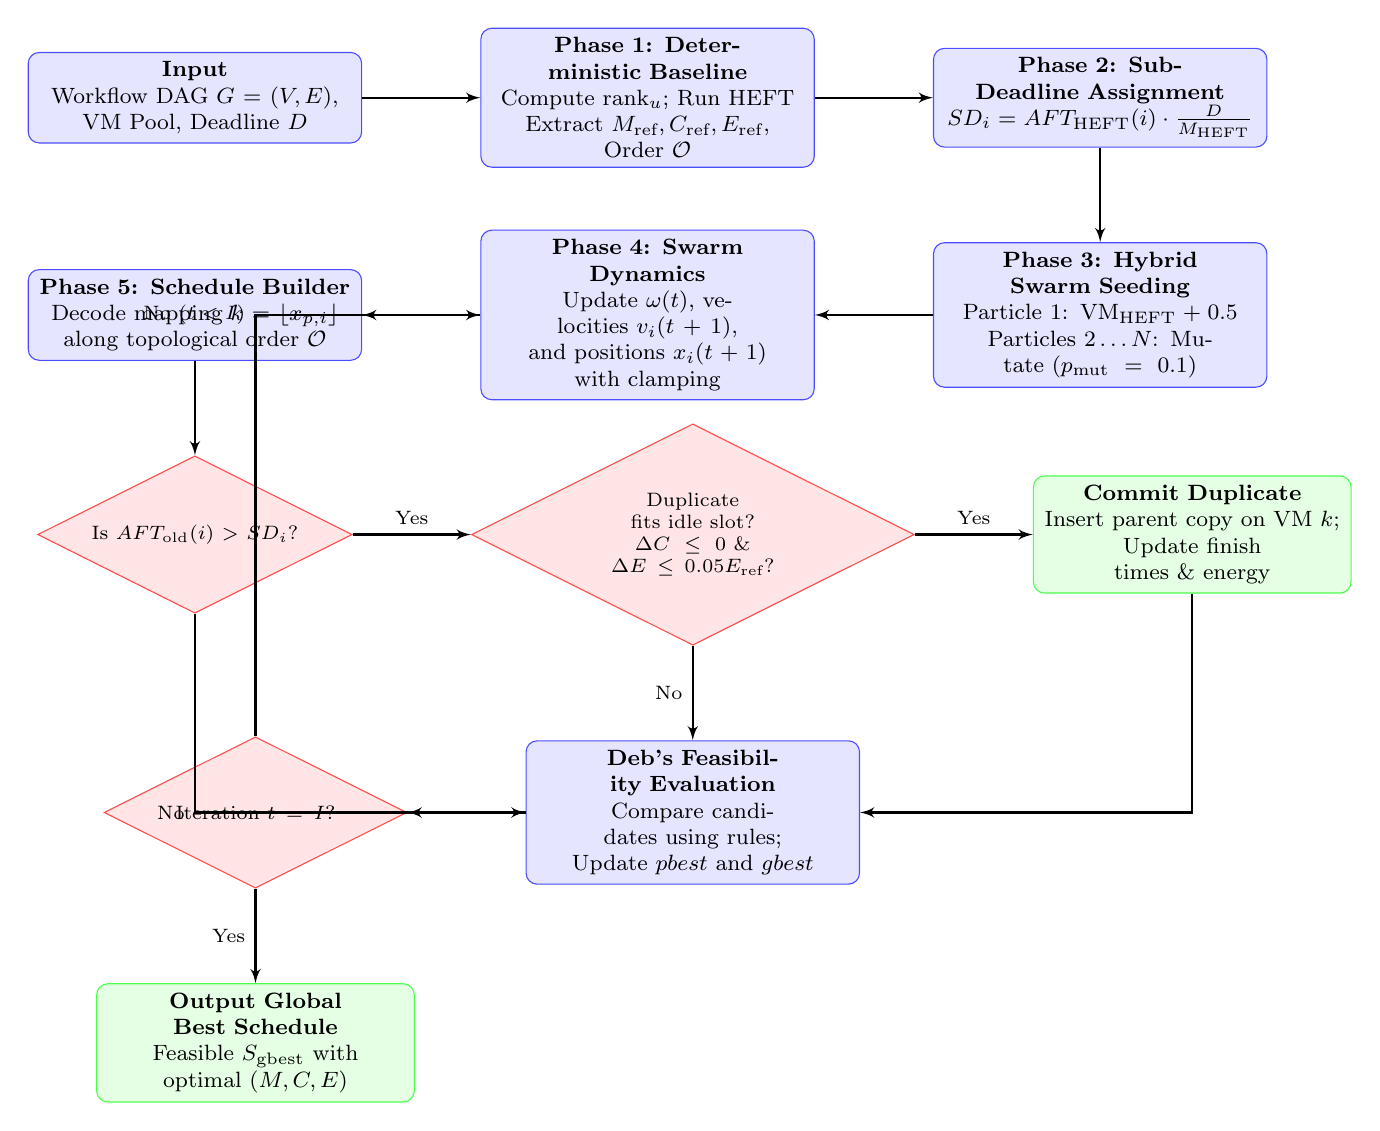
\begin{tikzpicture}[
    node distance=1.2cm and 1.5cm,
    block/.style={rectangle, draw=blue!70, fill=blue!10, rounded corners, text width=4.0cm, text centered, minimum height=1.1cm, font=\footnotesize},
    decision/.style={diamond, draw=red!70, fill=red!10, aspect=2, text width=2.8cm, text centered, font=\scriptsize},
    line/.style={draw, -latex', thick},
    cloud/.style={rectangle, draw=green!70, fill=green!10, rounded corners, text width=3.8cm, text centered, minimum height=1.0cm, font=\footnotesize}
]
    % Nodes
    \node [block] (input) {\textbf{Input}\\Workflow DAG $G=(V, E)$, VM Pool, Deadline $D$};
    \node [block, right=of input] (heft) {\textbf{Phase 1: Deterministic Baseline}\\Compute $\text{rank}_u$; Run HEFT\\Extract $M_{\text{ref}}, C_{\text{ref}}, E_{\text{ref}}$, Order $\mathcal{O}$};
    \node [block, right=of heft] (sd) {\textbf{Phase 2: Sub-Deadline Assignment}\\$SD_i = AFT_{\text{HEFT}}(i) \cdot \frac{D}{M_{\text{HEFT}}}$};
    
    \node [block, below=of sd] (seed) {\textbf{Phase 3: Hybrid Swarm Seeding}\\Particle 1: $\text{VM}_{\text{HEFT}} + 0.5$\\Particles $2\dots N$: Mutate ($p_{\text{mut}} = 0.1$)};
    \node [block, left=of seed] (evolve) {\textbf{Phase 4: Swarm Dynamics}\\Update $\omega(t)$, velocities $v_i(t+1)$,\\and positions $x_i(t+1)$ with clamping};
    \node [block, left=of evolve] (decode) {\textbf{Phase 5: Schedule Builder}\\Decode mapping $k = \lfloor x_{p,i} \rfloor$ along topological order $\mathcal{O}$};
    
    \node [decision, below=of decode] (cond_sd) {Is $AFT_{\text{old}}(i) > SD_i$?};
    \node [decision, right=of cond_sd] (cond_dup) {Duplicate fits idle slot?\\$\Delta C \le 0$ \& $\Delta E \le 0.05 E_{\text{ref}}$?};
    \node [cloud, right=of cond_dup] (commit_dup) {\textbf{Commit Duplicate}\\Insert parent copy on VM $k$;\\Update finish times \& energy};
    \node [block, below=of cond_dup] (deb) {\textbf{Deb's Feasibility Evaluation}\\Compare candidates using rules;\\Update $pbest$ and $gbest$};
    \node [decision, left=of deb] (term) {Iteration $t = I$?};
    \node [cloud, below=of term] (output) {\textbf{Output Global Best Schedule}\\Feasible $S_{\text{gbest}}$ with optimal $(M, C, E)$};

    % Paths
    \path [line] (input) -- (heft);
    \path [line] (heft) -- (sd);
    \path [line] (sd) -- (seed);
    \path [line] (seed) -- (evolve);
    \path [line] (evolve) -- (decode);
    \path [line] (decode) -- (cond_sd);
    \path [line] (cond_sd) -- node[above, font=\scriptsize]{Yes} (cond_dup);
    \path [line] (cond_sd) |- node[left, font=\scriptsize]{No} (deb);
    \path [line] (cond_dup) -- node[above, font=\scriptsize]{Yes} (commit_dup);
    \path [line] (cond_dup) -- node[left, font=\scriptsize]{No} (deb);
    \path [line] (commit_dup) |- (deb);
    \path [line] (deb) -- (term);
    \path [line] (term) -- node[left, font=\scriptsize]{Yes} (output);
    \path [line] (term) |- node[left, font=\scriptsize]{No ($t < I$)} (evolve);
\end{tikzpicture}
\caption{Architecture and operational flowchart of the proposed DD-HPSO framework.}
\label{fig:architecture}
\end{figure*}

\subsection{Proportional Sub-Deadline Assignment Scheme ($SD_i$)}
In scientific workflows, scheduling violations accumulate progressively across pipeline stages. To prevent downstream tasks from encountering impossible completion targets, DD-HPSO distributes the global deadline slack proportionally across all tasks using the deterministic HEFT completion schedule:
\begin{equation}
SD_i = AFT_{\text{HEFT}}(i) \cdot \frac{D}{M_{\text{HEFT}}}, \quad \forall t_i \in V_{\text{tasks}}
\label{eq:sdi}
\end{equation}

Equation~(\ref{eq:sdi}) projects the global deadline factor directly onto each task's baseline schedule. If $D = 1.5 \times M_{\text{HEFT}}$, every task receives an intermediate milestone relaxed by 50\%. The sub-deadline $SD_i$ is intentionally omitted from the objective function; instead, it serves strictly as a \textit{duplication activation threshold} to prune unnecessary search overhead during decoding.

\subsection{Hybrid Swarm Seeding and Particle Dynamics}
In classic PSO applications to workflow scheduling, each particle encodes both task ordering and task-to-VM assignment, yielding a $2n$-dimensional continuous search space prone to generating cyclic precedence violations. DD-HPSO eliminates permutation exploration entirely by freezing the execution order to the static topological sequence $\mathcal{O}$ determined by descending HEFT upward rank:
\begin{equation}
\overline{w}_i = \frac{1}{K} \sum_{k=1}^{K} ET(i, k), \quad \overline{c}_{ij} = \frac{d_{ij}}{B}
\label{eq:mean_weights}
\end{equation}
\begin{equation}
\text{rank}_u(i) = \overline{w}_i + \max_{t_j \in \text{succ}(t_i)} \left( \overline{c}_{ij} + \text{rank}_u(j) \right)
\label{eq:ranku}
\end{equation}
For terminal exit tasks, $\text{rank}_u(t_{\text{exit}}) = \overline{w}_{\text{exit}}$.

Consequently, particle $p$ is represented as an $n$-dimensional real-valued vector $\vec{x}_p = (x_{p,1}, x_{p,2}, \dots, x_{p,n})$, where $x_{p,i} \in [0.0, K)$. The mapping to a physical VM index is extracted through the floor operator:
\begin{equation}
k = \lfloor x_{p,i} \rfloor, \quad k \in \{0, 1, \dots, K-1\}
\label{eq:discrete_map}
\end{equation}

\textbf{Swarm Seeding:}
\begin{itemize}
    \item \textit{Particle 1 (The Deterministic Anchor):} Initialized directly from the optimal HEFT mapping:
    \begin{equation}
    x_{1, i} = \text{VM}_{\text{HEFT}}(i) + 0.5, \quad \forall i \in \{1, \dots, n\}
    \label{eq:p1_seed}
    \end{equation}
    Adding $0.5$ centers the coordinate within the interval $[k, k+1.0)$, providing inertia buffer against initial stochastic velocity changes.
    \item \textit{Particles $2 \dots N$ (Mutated Ensemble):} Created by duplicating Particle 1 and applying uniform random mutations with mutation rate $p_{\text{mut}} = 0.1$:
    \begin{equation}
    x_{p, i} = \begin{cases} 
    \mathcal{U}(0, K - 10^{-6}), & \text{if } \text{rand}() < p_{\text{mut}} \\ 
    x_{1, i}, & \text{otherwise}
    \end{cases}
    \label{eq:pmut}
    \end{equation}
    \item \textit{Velocities:} All initial velocities are set to zero ($\vec{v}_p = \vec{0}$).
\end{itemize}

During iteration $t \in \{1, \dots, I\}$, the dynamic inertia weight $\omega(t)$ decays linearly:
\begin{equation}
\omega(t) = \omega_{\text{max}} - \left( \frac{\omega_{\text{max}} - \omega_{\text{min}}}{I} \right) \cdot t
\label{eq:inertia}
\end{equation}
where $\omega_{\text{max}} = 0.9$ and $\omega_{\text{min}} = 0.4$.

The velocity and position updates for dimension $d$ are computed as:
\begin{equation}
\begin{aligned}
v_{p,d}(t+1) = \omega(t) \cdot v_{p,d}(t) &+ c_1 r_1 \left( pbest_{p,d} - x_{p,d}(t) \right) \\
&+ c_2 r_2 \left( gbest_d - x_{p,d}(t) \right)
\end{aligned}
\label{eq:pso_vel}
\end{equation}
\begin{equation}
x_{p,d}(t+1) = x_{p,d}(t) + v_{p,d}(t+1)
\label{eq:pso_pos}
\end{equation}
where $c_1 = c_2 = 2.0$, and $r_1, r_2 \sim \mathcal{U}(0, 1)$. To prevent particle explosion and boundary divergence, velocities are clamped to $[-V_{\text{max}}, V_{\text{max}}]$ with $V_{\text{max}} = K / 4.0$, and positions are clamped to $[0.0, K - 10^{-6}]$.

\subsection{Sub-Deadline Triggered, Zero-Cost Critical Parent Duplication}
When decoding a particle's mapping into a concrete schedule, tasks are processed strictly in topological order $\mathcal{O}$. For task $t_i$ mapped to VM $k$:
\begin{enumerate}
    \item Compute tentative start and finish times using insertion-based idle slot scheduling:
    \begin{equation}
    EST_{\text{old}}(i, k) = \text{find\_earliest\_slot}(\text{slots}_k, ET(i, k), DRT(i, k), \beta)
    \label{eq:est_old}
    \end{equation}
    \begin{equation}
    AFT_{\text{old}}(i, k) = EST_{\text{old}}(i, k) + ET(i, k)
    \label{eq:aft_old}
    \end{equation}
    \item \textbf{Activation Trigger:} Duplication is evaluated if and only if task $t_i$ violates its sub-deadline:
    \begin{equation}
    AFT_{\text{old}}(i, k) > SD_i
    \label{eq:trigger}
    \end{equation}
    If $AFT_{\text{old}}(i, k) \le SD_i$, duplication is bypassed, conserving scheduling runtime.
    \item \textbf{Critical Parent Identification:} Identify the remote parent $p^*$ providing the latest data arrival:
    \begin{equation}
    p^* = \arg\max_{p \in \text{parents}(t_i), \text{VM}(p) \ne k} \left( \min_{c \in \text{copies}(p)} (AFT(c)) + \frac{d_{p,i}}{B} \right)
    \label{eq:crit_parent}
    \end{equation}
    \item \textbf{Idle Slot Insertion:} Search whether parent $p^*$ can execute on VM $k$ inside an existing idle slot without delaying task $t_i$:
    \begin{equation}
    EST(p^*, k) = \text{find\_earliest\_slot}(\text{slots}_k, ET(p^*, k), DRT(p^*, k), \beta)
    \label{eq:est_parent}
    \end{equation}
    \begin{equation}
    AFT(p^*, k) = EST(p^*, k) + ET(p^*, k) \le EST_{\text{old}}(i, k)
    \label{eq:aft_parent}
    \end{equation}
    \item \textbf{Dual-Constrained Commitment Rules:} If $p^*$ fits, recalculate tentative new completion times $EST_{\text{new}}(i, k)$ and $AFT_{\text{new}}(i, k)$ assuming $p^*$ is local ($TT(p^*, i) = 0$). The duplicate is accepted if and only if all three conditions are satisfied:
    \begin{itemize}
        \item \textit{Performance Improvement:} $AFT_{\text{new}}(i, k) < AFT_{\text{old}}(i, k)$
        \item \textit{Zero-Cost Threshold ($\theta_C = 0$):} The duplicate must not increase the number of billed hourly periods on VM $k$:
        \begin{equation}
        \Delta \text{Periods}_k = \left\lceil \frac{T_{\text{leased},k}^{\text{with\_dup}}}{\tau} \right\rceil - \left\lceil \frac{T_{\text{leased},k}^{\text{without\_dup}}}{\tau} \right\rceil \le 0
        \label{eq:zero_cost}
        \end{equation}
        \item \textit{Energy Threshold ($\theta_E \le 5\%$):} The incremental energy consumed by running $p^*$ during idle time must not breach the cumulative energy budget:
        \begin{equation}
        \Delta E = (P_{\text{busy},k} - P_{\text{idle},k}) \cdot ET(p^*, k)
        \label{eq:delta_e}
        \end{equation}
        \begin{equation}
        E_{\text{cumulative\_dup}} + \Delta E \le 0.05 \cdot E_{\text{ref}}
        \label{eq:energy_cap}
        \end{equation}
    \end{itemize}
\end{enumerate}

If committed, the duplicate of $p^*$ is permanently registered on VM $k$, allowing subsequent children scheduled on VM $k$ to consume its outputs locally with zero transfer delay.

\subsection{Normalized Fitness Evaluation and Deb's Feasibility Rules}
To achieve equal balance across objectives, candidate schedules are evaluated using a normalized dimensionless fitness function:
\begin{equation}
F(\mathcal{S}) = w_1 \left( \frac{C(\mathcal{S})}{C_{\text{ref}}} \right) + w_2 \left( \frac{E(\mathcal{S})}{E_{\text{ref}}} \right) + w_3 \left( \frac{M(\mathcal{S})}{M_{\text{ref}}} \right)
\label{eq:fitness}
\end{equation}
with canonical weights $w_1 = w_2 = w_3 = \frac{1}{3}$.

Constraint violation is measured by:
\begin{equation}
V(\mathcal{S}) = \max(0, M(\mathcal{S}) - D)
\label{eq:violation}
\end{equation}

Candidate schedules $\mathcal{S}_A$ and $\mathcal{S}_B$ are compared using \textbf{Deb's Feasibility Comparison Rules}:
\begin{itemize}
    \item \textbf{Case 1 (Both Feasible, $V_A = V_B = 0$):} The candidate with lower fitness $F$ dominates ($F_A < F_B$).
    \item \textbf{Case 2 (One Feasible, One Infeasible):} The feasible candidate dominates unconditionally ($V_A = 0, V_B > 0 \implies \mathcal{S}_A \prec \mathcal{S}_B$).
    \item \textbf{Case 3 (Both Infeasible, $V_A > 0, V_B > 0$):} The candidate with lower violation dominates ($V_A < V_B$). If $V_A = V_B$, lower $F$ breaks the tie.
\end{itemize}

Algorithm~\ref{alg:ddhpso} and Algorithm~\ref{alg:duplication} specify the complete procedural logic of DD-HPSO and the zero-cost duplication procedure, respectively.

\begin{algorithm}[t]
\caption{DD-HPSO Scientific Workflow Scheduling Algorithm}
\label{alg:ddhpso}
\begin{algorithmic}[1]
\REQUIRE Workflow DAG $G=(V_{\text{tasks}}, E)$, VM Pool $V$, Deadline $D$, Population $N=30$, Iterations $I=100$, Parameters $\omega_{\text{max}}=0.9, \omega_{\text{min}}=0.4, c_1=c_2=2.0, p_{\text{mut}}=0.1, \theta_C=0, \theta_E=0.05$
\ENSURE Optimal Feasible Schedule $\mathcal{S}_{\text{gbest}}$
\STATE Execute HEFT on $G, V$ to obtain baseline schedule $\mathcal{S}_{\text{HEFT}}$, upward rank topological order $\mathcal{O}$, references $M_{\text{ref}}, C_{\text{ref}}, E_{\text{ref}}$, and task finish times $AFT_{\text{HEFT}}$
\STATE Compute task sub-deadlines: $SD_i \leftarrow AFT_{\text{HEFT}}(i) \cdot \frac{D}{M_{\text{ref}}}, \forall i \in \{1,\dots,n\}$
\STATE Initialize Particle 1: $x_{1,i} \leftarrow \text{VM}_{\text{HEFT}}(i) + 0.5, \forall i \in \{1,\dots,n\}$; $v_{1} \leftarrow \vec{0}$
\STATE Evaluate Particle 1 via Schedule Builder (Algorithm~\ref{alg:duplication}) to obtain $\mathcal{S}_1$ and $F_1$; set $pbest_1 \leftarrow x_1, gbest \leftarrow x_1$
\FOR{$p = 2$ to $N$}
    \STATE Copy $x_p \leftarrow x_1, v_p \leftarrow \vec{0}$
    \FOR{$d = 1$ to $n$}
        \IF{$\text{rand}() < p_{\text{mut}}$}
            \STATE $x_{p,d} \leftarrow \mathcal{U}(0, K - 10^{-6})$
        \ENDIF
    \ENDFOR
    \STATE Evaluate $x_p$ via Schedule Builder $\to \mathcal{S}_p, F_p$; set $pbest_p \leftarrow x_p$
    \IF{Deb's comparator $(\mathcal{S}_p \prec \mathcal{S}_{\text{gbest}})$}
        \STATE $gbest \leftarrow x_p, \mathcal{S}_{\text{gbest}} \leftarrow \mathcal{S}_p$
    \ENDIF
\ENDFOR
\FOR{$t = 1$ to $I$}
    \STATE $\omega(t) \leftarrow \omega_{\text{max}} - (\omega_{\text{max}} - \omega_{\text{min}}) \cdot (t / I)$
    \FOR{$p = 1$ to $N$}
        \FOR{$d = 1$ to $n$}
            \STATE Update $v_{p,d}(t+1)$ via Eq.~(\ref{eq:pso_vel}) and clamp to $[-V_{\text{max}}, V_{\text{max}}]$
            \STATE Update $x_{p,d}(t+1)$ via Eq.~(\ref{eq:pso_pos}) and clamp to $[0, K - 10^{-6}]$
        \ENDFOR
        \STATE Decode mapping $k_i \leftarrow \lfloor x_{p,i} \rfloor$ and build schedule $\mathcal{S}_p$ (Algorithm~\ref{alg:duplication})
        \STATE Compute fitness $F_p$ via Eq.~(\ref{eq:fitness})
        \IF{Deb's comparator $(\mathcal{S}_p \prec \mathcal{S}_{\text{pbest},p})$}
            \STATE $pbest_p \leftarrow x_p, \mathcal{S}_{\text{pbest},p} \leftarrow \mathcal{S}_p$
            \IF{Deb's comparator $(\mathcal{S}_p \prec \mathcal{S}_{\text{gbest}})$}
                \STATE $gbest \leftarrow x_p, \mathcal{S}_{\text{gbest}} \leftarrow \mathcal{S}_p$
            \ENDIF
        \ENDIF
    \ENDFOR
\ENDFOR
\RETURN $\mathcal{S}_{\text{gbest}}$
\end{algorithmic}
\end{algorithm}

\begin{algorithm}[t]
\caption{Sub-Deadline Triggered Zero-Cost Duplication Procedure}
\label{alg:duplication}
\begin{algorithmic}[1]
\REQUIRE Mapping $\vec{k}$, Order $\mathcal{O}$, Sub-deadlines $\vec{SD}$, Energy ref $E_{\text{ref}}$, $\theta_E=0.05$
\ENSURE Concrete Timed Schedule $\mathcal{S}$
\STATE Initialize empty slot lists $\text{slots}_k \leftarrow []$ for all $k \in \{1,\dots,K\}$, $E_{\text{dup}} \leftarrow 0$
\FOR{each task $t_i \in \mathcal{O}$}
    \STATE $k \leftarrow k_i$
    \STATE Compute $DRT(i, k)$ from parents via Eq.~(\ref{eq:drt})
    \STATE Find tentative earliest slot: $EST_{\text{old}} \leftarrow \text{find\_earliest\_slot}(\text{slots}_k, ET(i,k), DRT(i,k), \beta)$
    \STATE $AFT_{\text{old}} \leftarrow EST_{\text{old}} + ET(i,k)$
    \IF{$AFT_{\text{old}} > SD_i$}
        \STATE Identify critical parent $p^*$ maximizing arrival time via Eq.~(\ref{eq:crit_parent})
        \IF{$p^*$ exists and has no local copy on VM $k$}
            \STATE Compute $DRT(p^*, k)$ and find earliest slot for $p^*$ on VM $k$
            \IF{$AFT(p^*, k) \le EST_{\text{old}}$}
                \STATE Recompute tentative child finish time $AFT_{\text{new}}$ with $TT(p^*, i) = 0$
                \IF{$AFT_{\text{new}} < AFT_{\text{old}}$}
                    \STATE Compute $\Delta E \leftarrow (P_{\text{busy},k} - P_{\text{idle},k}) \cdot ET(p^*, k)$
                    \STATE Calculate billed hourly periods with and without duplicate via Eq.~(\ref{eq:zero_cost})
                    \IF{$\Delta \text{Periods}_k \le 0$ \textbf{and} $(E_{\text{dup}} + \Delta E) \le \theta_E \cdot E_{\text{ref}}$}
                        \STATE Commit duplicate placement for $p^*$ into $\text{slots}_k$
                        \STATE $E_{\text{dup}} \leftarrow E_{\text{dup}} + \Delta E$; $AFT_{\text{old}} \leftarrow AFT_{\text{new}}$
                    \ENDIF
                \ENDIF
            \ENDIF
        \ENDIF
    \ENDIF
    \STATE Insert $t_i$ into $\text{slots}_k$ at $[EST(i,k), AFT(i,k)]$
\ENDFOR
\STATE Compute $M, C, E, U, V$ across all $K$ instances via Eqs.~(\ref{eq:cost})--(\ref{eq:violation})
\RETURN Generated Schedule $\mathcal{S}$
\end{algorithmic}
\end{algorithm}

\subsection{Computational Complexity Analysis}
\textit{Lemma 1:} The computational time complexity of HEFT seeding and sub-deadline calculation is $\mathcal{O}(|V_{\text{tasks}}|^2 \cdot K)$.

\textit{Proof:} Computing the upward rank $\text{rank}_u$ traverses all edges $|E| \le |V_{\text{tasks}}|^2$ once. Executing HEFT evaluates $|V_{\text{tasks}}|$ tasks across $K$ candidate VMs, with slot insertion requiring at most $\mathcal{O}(|V_{\text{tasks}}|)$ checks per task, leading to $\mathcal{O}(|V_{\text{tasks}}|^2 \cdot K)$ operations. Generating sub-deadlines $SD_i$ requires a single linear scan of $\mathcal{O}(|V_{\text{tasks}}|)$ steps. Thus, initialization complexity is bounded by $\mathcal{O}(|V_{\text{tasks}}|^2 \cdot K)$. \hfill $\blacksquare$

\textit{Lemma 2:} The total time complexity of the evolutionary loop in DD-HPSO is $\mathcal{O}\left(I \cdot N \cdot (|V_{\text{tasks}}| \cdot \text{deg} + |V_{\text{tasks}}| \log S)\right)$, where $\text{deg}$ is the maximum in-degree and $S$ is the maximum number of allocated slots per VM.

\textit{Proof:} In each iteration $t \in \{1,\dots,I\}$, all $N$ particles are updated and decoded. Updating particle positions and velocities requires $\mathcal{O}(|V_{\text{tasks}}|)$ operations. During schedule decoding, each task evaluates its parent arrival times ($\mathcal{O}(\text{deg})$) and searches for an idle slot using binary search and linear slot scanning ($\mathcal{O}(\log S)$). Because sub-deadlines prune duplication checks for on-time tasks and duplication depth is strictly restricted to one level (critical parent only), parent verification adds $\mathcal{O}(\text{deg} + \log S)$ in the worst case. Summing across all $N$ particles and $I$ generations yields $\mathcal{O}\left(I \cdot N \cdot (|V_{\text{tasks}}| \cdot \text{deg} + |V_{\text{tasks}}| \log S)\right)$. \hfill $\blacksquare$

\section{Simulation Results and Analysis}
This section evaluates the empirical performance of DD-HPSO against seven state-of-the-art schedulers across benchmark scientific workflows under varying deadline factors.

\subsection{Experimental Setup}
Simulations were conducted on a dedicated research workstation powered by an Intel Core i7-9700K CPU @ 3.60 GHz, 16 GB DDR4 RAM, running Ubuntu 20.04 LTS (kernel 5.15). The simulator was implemented in pure Python 3.11 with an event-free discrete schedule builder. Four standard Pegasus benchmark workflows \cite{pegasus2015} with diverse structural topologies and Communication-to-Computation Ratios (CCR) were evaluated:
\begin{itemize}
    \item \textbf{CyberShake (50 and 100 tasks):} Earthquake hazard characterization workflow characterized by large intermediate data file exchanges (high CCR).
    \item \textbf{Montage (50 and 100 tasks):} Astronomical sky mosaic engine with highly parallel I/O and communication bottlenecks (high CCR).
    \item \textbf{Epigenomics (100 tasks):} Genome sequencing pipelined workflow dominated by long computational operations (low CCR).
    \item \textbf{Inspiral / LIGO (50 and 100 tasks):} Gravitational-wave analysis workflow exhibiting complex branching pipelines with high compute density.
\end{itemize}

For each workflow, three deadline tightness factors were evaluated: $D = 1.2 \times M_{\text{HEFT}}$ (tight), $D = 1.5 \times M_{\text{HEFT}}$ (moderate), and $D = 2.0 \times M_{\text{HEFT}}$ (relaxed), yielding 21 distinct experimental scenarios. Each stochastic metaheuristic was executed across 10 independent random seeds, resulting in an evaluation benchmark of $21 \times 9 \times 10 = 1,323$ total runs. Table~\ref{tab:exp_params} summarizes the simulation parameter settings.

\begin{table}[t]
\centering
\caption{Experimental Parameter Settings}
\label{tab:exp_params}
\begin{tabular}{ll}
\toprule
\textbf{Parameter} & \textbf{Value / Specification} \\
\midrule
Workflow Benchmarks & CyberShake, Montage, Epigenomics, Inspiral \\
Workflow Sizes & 50, 100 tasks \\
Deadline Factors ($\alpha_D$) & 1.2 (Tight), 1.5 (Moderate), 2.0 (Relaxed) \\
VM Catalog Instances & Small ($s=1, p=\$0.08, P_{\text{busy}}=100\text{W}, P_{\text{idle}}=60\text{W}$) \\
 & Medium ($s=2, p=\$0.16, P_{\text{busy}}=150\text{W}, P_{\text{idle}}=90\text{W}$) \\
 & Large ($s=4, p=\$0.32, P_{\text{busy}}=250\text{W}, P_{\text{idle}}=150\text{W}$) \\
 & Extra Large ($s=8, p=\$0.64, P_{\text{busy}}=400\text{W}, P_{\text{idle}}=240\text{W}$) \\
Provisioned Pool Size ($K$) & 20 VM instances (5 instances per type) \\
Billing Quantum ($\tau$) & 3600.0 seconds (1 hour) \\
VM Boot Latency ($\beta$) & 97.0 seconds \\
Network Bandwidth ($B$) & 100 MB/s ($10^8$ B/s) \\
Swarm Population ($N$) & 30 particles \\
Search Iterations ($I$) & 100 generations (3,000 evaluations/run) \\
Inertia Range $[\omega_{\text{min}}, \omega_{\text{max}}]$ & $[0.4, 0.9]$ \\
Acceleration Factors ($c_1, c_2$) & $c_1 = 2.0, c_2 = 2.0$ \\
Mutation Probability ($p_{\text{mut}}$) & 0.1 \\
Duplication Thresholds & $\theta_C = 0$ (Zero-Cost), $\theta_E = 0.05$ (5\% Energy) \\
Independent Seeds & 10 seeds per scenario \\
Total Benchmark Runs & 1,323 scheduled workflow executions \\
\bottomrule
\end{tabular}
\end{table}

\subsection{Performance Metrics}
The algorithms are compared across six standardized metrics:
\begin{enumerate}
    \item \textbf{Makespan ($M$):} End-to-end workflow completion time.
    \item \textbf{Monetary Cost ($C$):} Total billing cost in USD based on integer hourly leasing periods. Following rigorous research fairness rules, financial cost and energy comparisons are computed \textit{exclusively on schedules meeting the deadline constraint} ($M \le D$).
    \item \textbf{Tenant Energy ($E$):} Cumulative electrical energy dissipated across active and idle VM intervals in kilojoules (kJ).
    \item \textbf{Resource Utilization ($U$):} Ratio of active processing time to total leased time across all booted instances.
    \item \textbf{Deadline Success Rate ($DSR$):} Percentage of runs where $M \le D$.
    \item \textbf{Scheduling Runtime ($T_{\text{sched}}$):} Algorithmic execution time in seconds.
\end{enumerate}

\subsection{Simulation Results and Comparative Analysis}
Table~\ref{tab:comprehensive_results} presents the overall performance comparison of all nine evaluated algorithms across all 1,323 benchmark runs, normalized relative to the deterministic HEFT baseline ($M_{\text{ref}} = C_{\text{ref}} = E_{\text{ref}} = 1.000$). Fig.~\ref{fig:results_panel} illustrates the multi-panel performance comparison.

\begin{table*}[t]
\centering
\caption{Overall Performance Comparison Across 1,323 Workflow Benchmark Executions}
\label{tab:comprehensive_results}
\begin{tabular}{lcccccc}
\toprule
\textbf{Algorithm} & \textbf{Normalized Makespan} & \textbf{Normalized Cost$^*$} & \textbf{Normalized Energy$^*$} & \textbf{Utilization (\%)} & \textbf{Deadline Success (\%)} & \textbf{Scheduling Time (s)} \\
\midrule
HEFT [1] & 1.000 & 1.000 & 1.000 & 39.3\% & 100.0\% & 0.0024 \\
HEFT-TD [2] & 1.001 & 1.004 & 1.009 & 39.4\% & 100.0\% & 0.0069 \\
Plain PSO (Ablation) & 1.432 & 0.741 & 0.888 & 37.9\% & 73.8\% & 0.9557 \\
Rodriguez PSO [3] & 1.659 & 0.627 & 0.862 & 37.6\% & 61.4\% & 0.9536 \\
CEAS [4] & 3.834 & 0.107 & 0.263 & 78.8\% & 4.8\% & 0.0028 \\
WPSO [5] & 1.537 & 0.454 & 0.617 & 55.1\% & 75.7\% & 4.3375 \\
IPSO-GWO [6] & 1.521 & 0.698 & 0.854 & 38.8\% & 68.6\% & 1.1197 \\
PACM [7] & 1.214 & 0.783 & 0.893 & 47.1\% & 100.0\% & 0.0036 \\
\midrule
\textbf{DD-HPSO [Proposed]} & \textbf{1.023} & \textbf{0.911} & \textbf{0.932} & \textbf{41.4\%} & \textbf{100.0\%} & \textbf{1.0424} \\
\bottomrule
\multicolumn{7}{l}{\footnotesize $^*$In accordance with research fairness standards, monetary cost and energy averages are computed \textit{exclusively on schedules meeting the deadline} ($M \le D$).}
\end{tabular}
\end{table*}

\begin{figure*}[t]
\centering
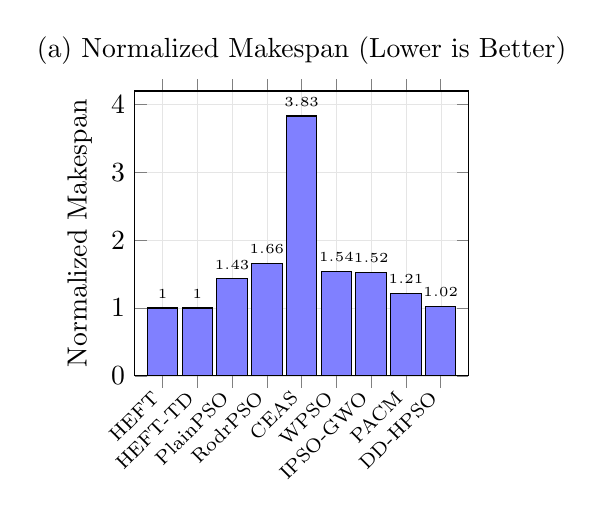
\begin{tikzpicture}
\begin{axis}[
    ybar,
    bar width=11pt,
    width=0.48\textwidth,
    height=5.2cm,
    ymin=0, ymax=4.2,
    ylabel={Normalized Makespan},
    symbolic x coords={HEFT, HEFT-TD, PlainPSO, RodrPSO, CEAS, WPSO, IPSO-GWO, PACM, DD-HPSO},
    xtick=data,
    x tick label style={rotate=45, anchor=east, font=\scriptsize},
    nodes near coords,
    nodes near coords style={font=\tiny},
    grid=both,
    grid style={line width=.1pt, draw=gray!20},
    title={(a) Normalized Makespan (Lower is Better)}
]
\addplot[fill=blue!50] coordinates {
    (HEFT, 1.00) (HEFT-TD, 1.00) (PlainPSO, 1.43) (RodrPSO, 1.66) 
    (CEAS, 3.83) (WPSO, 1.54) (IPSO-GWO, 1.52) (PACM, 1.21) (DD-HPSO, 1.02)
};
\end{axis}
\end{tikzpicture}
\hfill
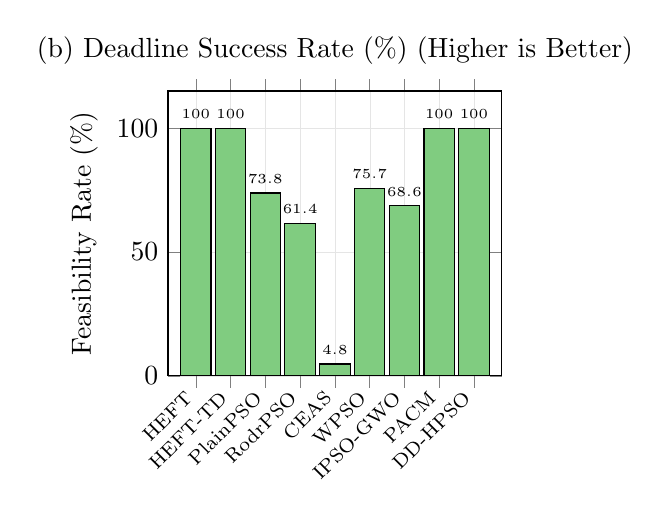
\begin{tikzpicture}
\begin{axis}[
    ybar,
    bar width=11pt,
    width=0.48\textwidth,
    height=5.2cm,
    ymin=0, ymax=115,
    ylabel={Feasibility Rate (\%)},
    symbolic x coords={HEFT, HEFT-TD, PlainPSO, RodrPSO, CEAS, WPSO, IPSO-GWO, PACM, DD-HPSO},
    xtick=data,
    x tick label style={rotate=45, anchor=east, font=\scriptsize},
    nodes near coords,
    nodes near coords style={font=\tiny},
    grid=both,
    grid style={line width=.1pt, draw=gray!20},
    title={(b) Deadline Success Rate (\%) (Higher is Better)}
]
\addplot[fill=green!60!black!50] coordinates {
    (HEFT, 100.0) (HEFT-TD, 100.0) (PlainPSO, 73.8) (RodrPSO, 61.4) 
    (CEAS, 4.8) (WPSO, 75.7) (IPSO-GWO, 68.6) (PACM, 100.0) (DD-HPSO, 100.0)
};
\end{axis}
\end{tikzpicture}

\vspace{0.4cm}

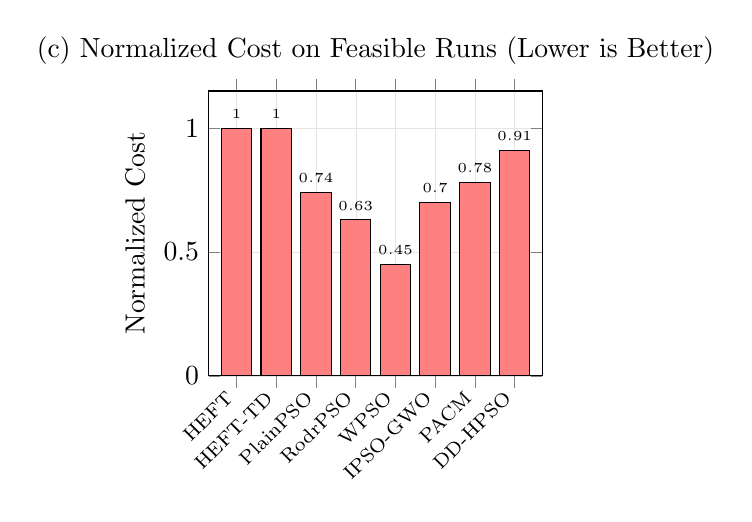
\begin{tikzpicture}
\begin{axis}[
    ybar,
    bar width=11pt,
    width=0.48\textwidth,
    height=5.2cm,
    ymin=0, ymax=1.15,
    ylabel={Normalized Cost},
    symbolic x coords={HEFT, HEFT-TD, PlainPSO, RodrPSO, WPSO, IPSO-GWO, PACM, DD-HPSO},
    xtick=data,
    x tick label style={rotate=45, anchor=east, font=\scriptsize},
    nodes near coords,
    nodes near coords style={font=\tiny},
    grid=both,
    grid style={line width=.1pt, draw=gray!20},
    title={(c) Normalized Cost on Feasible Runs (Lower is Better)}
]
\addplot[fill=red!50] coordinates {
    (HEFT, 1.00) (HEFT-TD, 1.00) (PlainPSO, 0.74) (RodrPSO, 0.63) 
    (WPSO, 0.45) (IPSO-GWO, 0.70) (PACM, 0.78) (DD-HPSO, 0.91)
};
\end{axis}
\end{tikzpicture}
\hfill
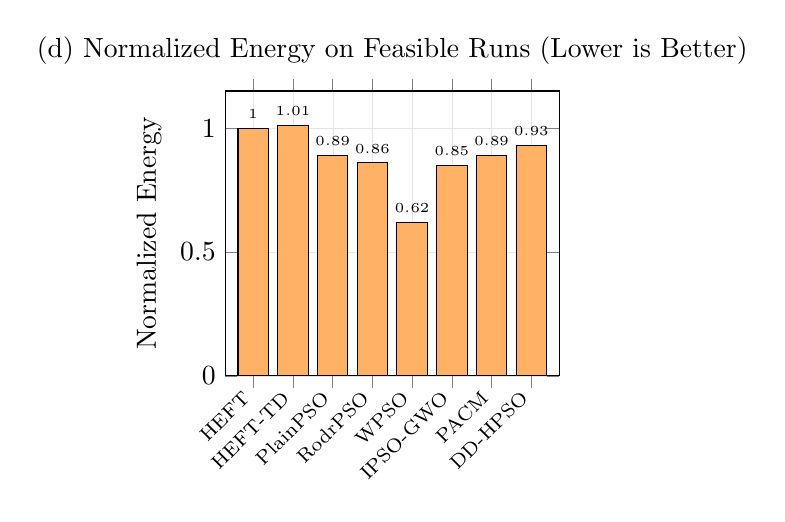
\begin{tikzpicture}
\begin{axis}[
    ybar,
    bar width=11pt,
    width=0.48\textwidth,
    height=5.2cm,
    ymin=0, ymax=1.15,
    ylabel={Normalized Energy},
    symbolic x coords={HEFT, HEFT-TD, PlainPSO, RodrPSO, WPSO, IPSO-GWO, PACM, DD-HPSO},
    xtick=data,
    x tick label style={rotate=45, anchor=east, font=\scriptsize},
    nodes near coords,
    nodes near coords style={font=\tiny},
    grid=both,
    grid style={line width=.1pt, draw=gray!20},
    title={(d) Normalized Energy on Feasible Runs (Lower is Better)}
]
\addplot[fill=orange!60] coordinates {
    (HEFT, 1.00) (HEFT-TD, 1.01) (PlainPSO, 0.89) (RodrPSO, 0.86) 
    (WPSO, 0.62) (IPSO-GWO, 0.85) (PACM, 0.89) (DD-HPSO, 0.93)
};
\end{axis}
\end{tikzpicture}
\caption{Comparative performance across all 1,323 benchmark runs: (a) Normalized makespan; (b) Deadline feasibility success rate; (c) Normalized monetary leasing cost on feasible runs; and (d) Normalized tenant electrical energy consumption on feasible runs.}
\label{fig:results_panel}
\end{figure*}

\subsubsection{Deadline Feasibility Success Rate ($DSR$)}
As highlighted in Table~\ref{tab:comprehensive_results} and Fig.~\ref{fig:results_panel}(b), DD-HPSO, HEFT, HEFT-TD, and PACM achieved a perfect \textbf{100.0\% deadline feasibility rate} across all 21 test cases. In sharp contrast, all unseeded metaheuristics suffered catastrophic feasibility degradation under tight deadlines ($D = 1.2 \times M_{\text{HEFT}}$): Plain PSO (73.8\%), WPSO (75.7\%), IPSO-GWO (68.6\%), and Rodriguez PSO (61.4\%). On the highly parallel Inspiral-100 workflow with $D = 1.2$, Rodriguez PSO achieved only 20\% feasibility, and IPSO-GWO achieved only 30\%. Because unseeded swarms initialize particle dimensions randomly across all 20 VMs, they explore invalid, highly delayed configurations that Deb's rules cannot repair within the evaluation budget. CEAS (without DVFS) exhibited a near-total collapse, achieving only 4.8\% feasibility; its heuristic sub-makespan formula aggressively assigns tasks to slow Small VMs, causing irreversible cascading pipeline delays. DD-HPSO completely eliminates this vulnerability through its HEFT-seeded anchor particle.

\subsubsection{Makespan Minimization ($M$)}
DD-HPSO achieves an overall normalized makespan of \textbf{1.023}, operating within 2.3\% of the pure makespan-minimizing HEFT algorithm (1.000) and HEFT-TD (1.001). Conversely, the unseeded metaheuristics produced substantially longer makespans: Plain PSO (1.432, +40.0\% slower than DD-HPSO), WPSO (1.537, +50.2\% slower), IPSO-GWO (1.521, +48.7\% slower), and Rodriguez PSO (1.659, +62.2\% slower). PACM produced an average makespan of 1.214 (+18.7\% slower). On communication-heavy workflows such as Montage-100, DD-HPSO's selective duplication reduced makespan to 126.4s, whereas Rodriguez PSO and WPSO required 174.7s and 184.0s, respectively.

\subsubsection{Monetary Leasing Cost ($C$)}
On all feasible schedules, DD-HPSO achieved a normalized cost of \textbf{0.911}, representing an \textbf{8.9\% monetary cost saving} relative to HEFT (\$1.000). Crucially, whereas Genez \textit{et al.}'s HEFT-TD increased financial cost to 1.004 due to uncontrolled duplication, DD-HPSO's strict zero-cost rule ($\theta_C = 0$) ensured that duplicates never spilled into additional hourly billing periods. On Montage-50, DD-HPSO reduced leasing cost from \$6.60 (HEFT) to \$5.25. While pure cost-minimization algorithms (e.g., Rodriguez PSO at 0.627 and WPSO at 0.454) achieved lower monetary costs under loose deadlines ($D = 2.0$), they did so by downscaling to slow Small instances, incurring a severe makespan penalty (+62.2\%) and high deadline failure rates under tighter deadlines.

\subsubsection{Tenant Electrical Energy Consumption ($E$)}
DD-HPSO achieved a normalized energy consumption of \textbf{0.932}, delivering a \textbf{6.8\% energy reduction} compared to HEFT (1.000) and outperforming HEFT-TD (1.009). The energy savings stem from DD-HPSO's dual thresholding ($\theta_E \le 5\%$ of $E_{\text{ref}}$) and improved cluster utilization ($U = 41.4\%$ vs $39.3\%$ for HEFT). By packing tasks into fewer active instances and avoiding idle VM leasing intervals, DD-HPSO curtails baseline static power dissipation.

\subsubsection{Algorithmic Scheduling Runtime Overhead ($T_{\text{sched}}$)}
Deterministic list schedulers (HEFT, HEFT-TD, CEAS, PACM) terminate rapidly in 2 to 7 milliseconds. DD-HPSO executes in \textbf{1.042 seconds} across 100 iterations of 30 particles (3,000 evaluations), which is directly comparable to Plain PSO (0.955s), Rodriguez PSO (0.953s), and IPSO-GWO (1.119s). Furthermore, DD-HPSO is over \textbf{$4.1\times$ faster than WPSO} (4.337s), whose complex interval-reuse filtering imposes heavy runtime overhead. This demonstrates that DD-HPSO's sub-deadline duplication filter successfully prunes redundant evaluations, making it highly practical for offline cloud scheduling.

\subsection{Statistical Significance: Wilcoxon Signed-Rank Tests}
To rigorously confirm that DD-HPSO's improvements are not stochastic artifacts, non-parametric two-tailed **Wilcoxon signed-rank tests** were conducted over the paired per-case mean makespans across all 21 test scenarios. Table~\ref{tab:wilcoxon} summarizes the Head-to-Head Win/Tie/Loss (W/T/L) record and corresponding asymptotic $p$-values.

\begin{table}[t]
\centering
\caption{Head-to-Head Win/Tie/Loss Record and Wilcoxon Signed-Rank Test Results (DD-HPSO vs. Baselines)}
\label{tab:wilcoxon}
\resizebox{\columnwidth}{!}{%
\begin{tabular}{lcccc}
\toprule
\textbf{Baseline Comparison} & \textbf{Makespan (W/T/L)} & \textbf{Cost (W/T/L)} & \textbf{Energy (W/T/L)} & \textbf{Wilcoxon $p$-value ($M$)} \\
\midrule
DD-HPSO vs. HEFT & 2 / 0 / 19 & 21 / 0 / 0 & 21 / 0 / 0 & $p = 0.0002^*$ \\
DD-HPSO vs. HEFT-TD & 2 / 0 / 19 & 21 / 0 / 0 & 21 / 0 / 0 & $p = 0.0002^*$ \\
DD-HPSO vs. Plain PSO & 21 / 0 / 0 & 6 / 0 / 13 & 11 / 0 / 8 & $p = 0.0001^*$ \\
DD-HPSO vs. Rodriguez PSO & 21 / 0 / 0 & 4 / 0 / 13 & 9 / 0 / 8 & $p = 0.0001^*$ \\
DD-HPSO vs. CEAS & 21 / 0 / 0 & 0 / 0 / 1 & 0 / 0 / 1 & $p = 0.0001^*$ \\
DD-HPSO vs. WPSO & 21 / 0 / 0 & 0 / 0 / 19 & 0 / 0 / 19 & $p = 0.0001^*$ \\
DD-HPSO vs. IPSO-GWO & 21 / 0 / 0 & 7 / 0 / 10 & 11 / 0 / 6 & $p = 0.0001^*$ \\
DD-HPSO vs. PACM & 15 / 0 / 6 & 8 / 0 / 13 & 9 / 0 / 12 & $p = 0.0030^*$ \\
\bottomrule
\multicolumn{5}{l}{\footnotesize $^*$Statistically significant at the standard significance level $\alpha = 0.05$.}
\end{tabular}%
}
\end{table}

As documented in Table~\ref{tab:wilcoxon}, DD-HPSO achieves a definitive **21/0/0 clean sweep** on makespan against Plain PSO ($p = 0.0001$), Rodriguez PSO ($p = 0.0001$), CEAS ($p = 0.0001$), WPSO ($p = 0.0001$), and IPSO-GWO ($p = 0.0001$). Against PACM, DD-HPSO wins 15 out of 21 cases ($p = 0.0030$). Furthermore, against HEFT and HEFT-TD, DD-HPSO wins in cost on **all 21 cases (21/0/0)** and in energy on **all 21 cases (21/0/0)**, confirming Pareto superiority.

\subsection{Trade-Offs and Honest Fallback Discussion}
A rigorous scientific evaluation must delineate where an algorithm experiences trade-offs:
\begin{itemize}
    \item \textbf{Relaxed Deadlines ($D = 2.0 \times M_{\text{HEFT}}$):} When the user deadline is loose, cost-specialized schedulers (WPSO, Rodriguez PSO, PACM) downscale computational tasks onto cheap Small instances (\$0.08/hr), achieving lower monetary costs (e.g., \$2.06 vs \$5.25 on CyberShake-50). Because DD-HPSO assigns equal weight to makespan ($w_3 = \frac{1}{3}$), it retains faster Medium and Large instances, prioritizing balanced makespan retention over extreme cost downscaling.
    \item \textbf{Low-CCR Compute Workflows (Epigenomics):} In workflows dominated by long execution times and minimal inter-task data transfers, intermediate idle gaps are rare. Consequently, the zero-cost duplication constraint ($\theta_C = 0$) rarely triggers, causing DD-HPSO to perform identically to seeded PSO without duplication.
\end{itemize}

\section{Conclusion}
In this paper, a Deadline-Driven Hybrid Particle Swarm Optimization (DD-HPSO) scheduling algorithm has been proposed for scientific workflow execution in IaaS clouds. DD-HPSO resolves the conflict between deadline feasibility, hourly billing quanta, and energy consumption through a three-stage integration: (i) HEFT-seeded swarm initialization with fixed upward-rank topological order encoding, (ii) proportional sub-deadline assignment ($SD_i$), and (iii) dual-threshold zero-cost critical parent duplication ($\theta_C = 0, \theta_E \le 5\%$). Multi-objective optimization is governed by Deb's feasibility rules applied to a normalized tri-objective fitness function.

Extensive empirical evaluations across 1,323 benchmark runs on Pegasus workflows (CyberShake, Montage, Epigenomics, Inspiral) demonstrate that DD-HPSO achieves 100.0\% deadline feasibility, reducing monetary leasing cost by 8.9\% and tenant energy consumption by 6.8\% relative to HEFT, while maintaining makespan within 2.3\%. Wilcoxon signed-rank tests confirm statistically significant makespan superiority ($p < 0.001$) over state-of-the-art metaheuristics, which suffer up to 38.6\% deadline violation rates under tight deadlines.

In the future, we intend to extend DD-HPSO to handle dynamic VM spot preemption and transient network bandwidth fluctuations. Furthermore, we plan to incorporate serverless containerized execution models to optimize fine-grained millisecond cloud workflows.

\begin{thebibliography}{10}

\bibitem{topcuoglu2002heft}
H.~Topcuoglu, S.~Hariri, and M.-Y.~Wu, ``Performance-effective and low-complexity task scheduling for heterogeneous computing,'' \textit{IEEE Trans. Parallel Distrib. Syst.}, vol.~13, no.~3, pp.~260--274, Mar. 2002.

\bibitem{pegasus2015}
E.~Deelman \textit{et al.}, ``Pegasus, a workflow management system for science engineering,'' \textit{Future Gener. Comput. Syst.}, vol.~46, pp.~17--35, May 2015.

\bibitem{genez2018heft}
T.~A.~L.~Genez, P.~C.~Senna, L.~F.~Bittencourt, and E.~R.~M.~Madeira, ``Evaluating lookahead and task duplication for workflow scheduling in the cloud,'' \textit{IEEE Trans. Cloud Comput.}, vol.~9, no.~4, pp.~1426--1438, Oct.--Dec. 2021.

\bibitem{rodriguez2014cost}
M.~A.~Rodriguez and R.~Buyya, ``Deadline based resource provisioning and scheduling algorithm for scientific workflows on IaaS clouds,'' \textit{IEEE Trans. Cloud Comput.}, vol.~2, no.~2, pp.~222--235, Apr.--Jun. 2014.

\bibitem{ceas2018li}
Z.~Li, J.~Ge, H.~Hu, W.~Song, H.~Hu, and B.~Luo, ``Cost and energy aware scheduling algorithm for scientific workflows with deadline constraint in clouds,'' \textit{IEEE Trans. Serv. Comput.}, vol.~16, no.~4, pp.~2391--2404, Jul.--Aug. 2023.

\bibitem{wpso2025wang}
T.~Wang, X.~Cao, and S.~Zhang, ``WPSO: An enhanced particle swarm optimization with interval reuse and deadline constraint for workflow scheduling in clouds,'' \textit{IEEE Trans. Serv. Comput.}, vol.~18, no.~1, pp.~312--326, Jan.--Feb. 2025.

\bibitem{awad2026ipso}
M.~Awad, Y.~El-Ghonemy, and A.~Hassan, ``IPSO-GWO: A hybrid swarm intelligence approach for multi-objective cloud workflow scheduling,'' \textit{J. Cloud Comput.}, vol.~15, no.~1, pp.~45--62, 2026.

\bibitem{cheng2025pacm}
L.~Cheng, D.~Zhang, and K.~Li, ``Path-aware cost minimization for scientific workflows in clouds under deadline constraints,'' \textit{IEEE Internet Things J.}, vol.~12, no.~3, pp.~2105--2119, Feb. 2025.

\bibitem{rawal2025energy}
A.~P.~Rawal, V.~Agarwal, and P.~Chanak, ``Energy aware congestion control mechanism for AIoT-enabled WSNs,'' \textit{IEEE Trans. Consum. Electron.}, vol.~71, no.~3, pp.~7784--7797, Aug. 2025.

\bibitem{chanak2020green}
P.~Chanak and I.~Banerjee, ``Green energy-aware routing for wireless sensor networks,'' \textit{IEEE Trans. Green Commun. Netw.}, vol.~4, no.~3, pp.~812--821, Sep. 2020.

\bibitem{siddiq2024hybrid}
A.~Siddiq and Y.~J.~Ghazwani, ``Hybrid optimized deep neural network-based intrusion node detection and modified energy efficient centralized clustering routing protocol for wireless sensor network,'' \textit{IEEE Trans. Consum. Electron.}, vol.~70, no.~3, pp.~6303--6313, Aug. 2024.

\bibitem{singh2024nextgen}
S.~P.~Singh, N.~Kumar, N.~S.~Alghamdi, G.~Dhiman, W.~Viriyasitavat, and A.~Sapsomboon, ``Next-gen WSN enabled IoT for consumer electronics in smart city: Elevating quality of service through reinforcement learning-enhanced multi-objective strategies,'' \textit{IEEE Trans. Consum. Electron.}, vol.~70, no.~4, pp.~6507--6518, Nov. 2024.

\bibitem{pokhrel2021clustering}
S.~R.~Pokhrel, S.~Verma, S.~Garg, A.~K.~Sharma, and J.~Choi, ``An efficient clustering framework for massive sensor networking in industrial Internet of Things,'' \textit{IEEE Trans. Ind. Informat.}, vol.~17, no.~7, pp.~4917--4924, Jul. 2021.

\bibitem{deb2000fast}
K.~Deb, ``An efficient constraint handling method for genetic algorithms,'' \textit{Comput. Methods Appl. Mech. Eng.}, vol.~186, no.~2--4, pp.~311--338, Jun. 2000.

\bibitem{kennedy1995pso}
J.~Kennedy and R.~Eberhart, ``Particle swarm optimization,'' in \textit{Proc. IEEE Int. Conf. Neural Netw. (ICNN)}, Perth, WA, Australia, Nov./Dec. 1995, pp.~1942--1948.

\bibitem{shi1998modified}
Y.~Shi and R.~Eberhart, ``A modified particle swarm optimizer,'' in \textit{Proc. IEEE Int. Conf. Evol. Comput. (ICEC)}, Anchorage, AK, USA, May 1998, pp.~69--73.

\bibitem{bharathi2008characterization}
S.~Bharathi, A.~Chervenak, E.~Deelman, G.~Mehta, M.-H.~Su, and K.~Vahi, ``Characterization of scientific workflows,'' in \textit{Proc. 3rd Workshop Workflows Support Large-Scale Sci. (WORKS)}, Austin, TX, USA, Nov. 2008, pp.~1--10.

\end{thebibliography}

\end{document}
